% $Header: /cvsroot/latex-beamer/latex-beamer/solutions/generic-talks/generic-ornate-15min-45min.en.tex,v 1.5 2007/01/28 20:48:23 tantau Exp $

\documentclass[letter,graphicx]{beamer}

% This file is a solution template for:

% - Giving a talk on some subject.
% - The talk is between 15min and 45min long.
% - Style is ornate.



% Copyright 2004 by Till Tantau <tantau@users.sourceforge.net>.
%
% In principle, this file can be redistributed and/or modified under
% the terms of the GNU Public License, version 2.
%
% However, this file is supposed to be a template to be modified
% for your own needs. For this reason, if you use this file as a
% template and not specifically distribute it as part of a another
% package/program, I grant the extra permission to freely copy and
% modify this file as you see fit and even to delete this copyright
% notice. 


\mode<presentation>
{
  \usetheme{Warsaw}
  % or ...

  \setbeamercovered{transparent}
  \setbeamertemplate{footling}[frame number]
  % or whatever (possibly just delete it)
}


\usepackage[english]{babel}
% or whatever

\usepackage[latin1]{inputenc}
% or whatever
\usepackage{verbatim}
\usepackage{times}
\usepackage[T1]{fontenc}
\def\Tiny{\fontsize{3pt}{3pt} \selectfont}
\def\ttiny{\fontsize{5pt}{5pt} \selectfont}
	
\logo{
\includegraphics[width=.1\textwidth]{./images/official_NOAA_logo.pdf}}

\title[SNP contamination identification with Bayesian methods\hspace{2em}\insertframenumber] % (optional, use only with long paper titles)
{Algorithms for Identifying Contaminated Samples Genotyped with Single Nucleotide Polymorphisms}

\subtitle{} % (optional)

\author[Elena Venable] % (optional, use only with lots of authors)
{Elena Venable}
% - Use the \inst{?} command only if the authors have different
%   affiliation.

\institute[Brown Univeristy] % (optional, but mostly needed)
{
Brown University \\ Applied Mathematics - Biology \\ Healthy Oceans \\ Southwest Fisheries Science Center, Santa Cruz, CA \\ Eric C. Anderson
}
% - Use the \inst command only if there are several affiliations.
% - Keep it simple, no one is interested in your street address.

\date[CSGM--2014] % (optional)
{
 Hollings and EPP Undergraduate Scholars Symposium \\ 29 AUGUST 2014}

\subject{Talks}
% This is only inserted into the PDF information catalog. Can be left
% out. 



% If you have a file called "university-logo-filename.xxx", where xxx
% is a graphic format that can be processed by latex or pdflatex,
% resp., then you can add a logo as follows:

% \pgfdeclareimage[height=0.5cm]{university-logo}{university-logo-filename}
% \logo{\pgfuseimage{university-logo}}

% Delete this, if you do not want the table of contents to pop up at
% the beginning of each subsection:
%\AtBeginSection[]
%{
%  \begin{frame}<beamer>{Outline}
%    \tableofcontents[currentsection,currentsubsection]
%  \end{frame}
%}
% If you wish to uncover everything in a step-wise fashion, uncomment
% the following command: 

%\beamerdefaultoverlayspecification{<+->}

%% More eric commands for inserting some small figures
%\newcommand{\smikid}{\includegraphics[width=3.7ex]{images/smiley_blue_kid.pdf}}
%\newcommand{\smired}{\includegraphics[width=2.9ex]{images/smiley_sad_red.png}}
%\newcommand{\smiblue}{\includegraphics[width=2.9ex]{images/smiley_happy_blue.png}}
%\newcommand{\thh}{^\mathrm{th}}
%\newcommand{\tc}{\textcolor}
%\def\bm#1{\mathpalette\bmstyle{#1}}
%\def\bmstyle#1#2{\mbox{\boldmath$#1#2$}}


\begin{document}

%Slide 1
\begin{frame}
  \titlepage
\end{frame}

%Slide 2
\begin{frame}{Overview}
   \begin{itemize}
	\item Introduction/Objectives
	\item Background Theory
	\item Single Population Model
	\item Mixture Model
	\item Conclusion
   \end{itemize}
\end{frame}

%Slide 3
\begin{frame}{Introduction/Objectives}
  \begin{columns}[T]
 
 \column{2.75 in}
 \centering 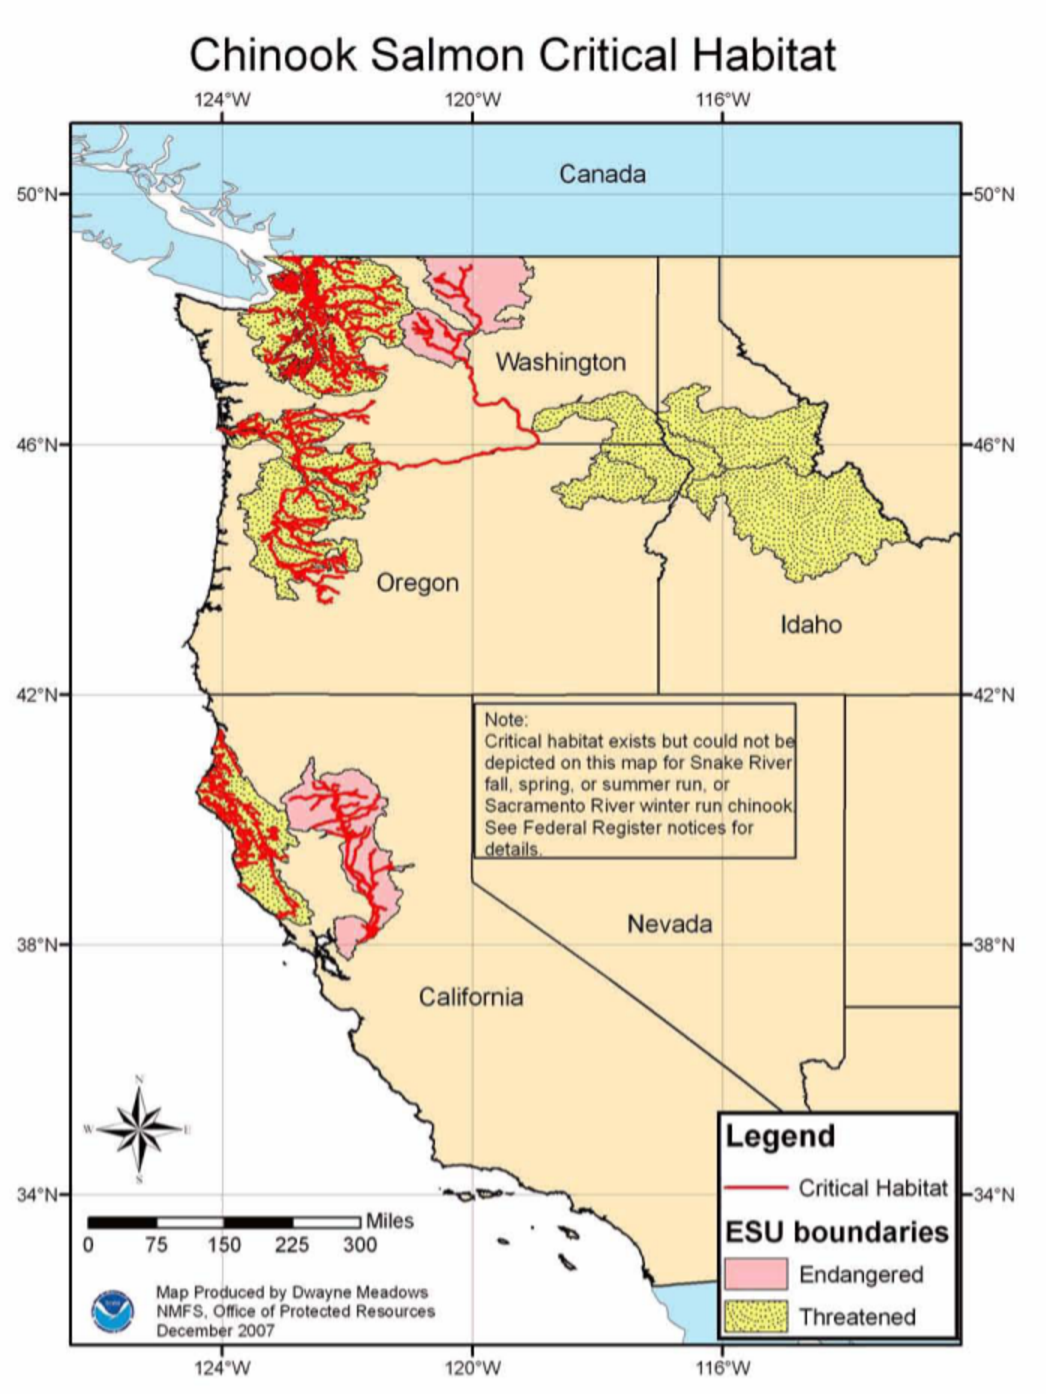
\includegraphics[width=.8\textwidth]{images/chinooksalmon} \\
\centering \Tiny \url{http://www.nmfs.noaa.gov/pr/species/fish/chinooksalmon.htm}	
 
  \column{2.25in}
   \begin{itemize}
	\item Importance of stock ID of West Coast salmon
		\vspace{2mm}
	\item New Single Nucleotide Polymorphism (SNP) technology
   \end{itemize}
   \vspace{2mm}
  \centering  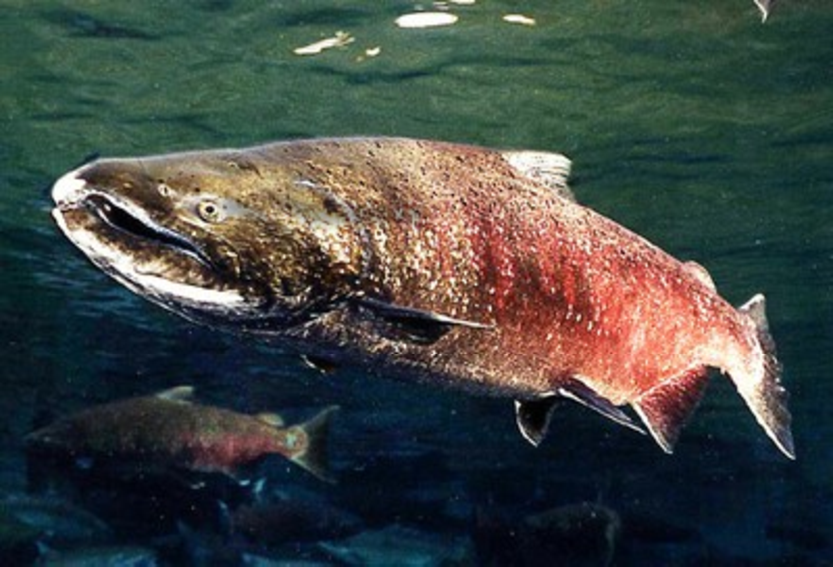
\includegraphics[width=.75\textwidth]{images/salmon_individual}
  \Tiny
  \url{http://www.wta.org/hiking-info/nature-on-trail/nature-on-trail-chinook-salmon}
   
   \end{columns}
\end{frame}

%Slide 4
\begin{frame}{Background Theory}
\framesubtitle{Single Nucleotide Polymorphisms (SNPs)}
\begin{itemize}
\item DNA sequence variation differing by a single base
\vspace{2mm}
\item most SNPs have only two alleles 
\end{itemize}
\begin{center}
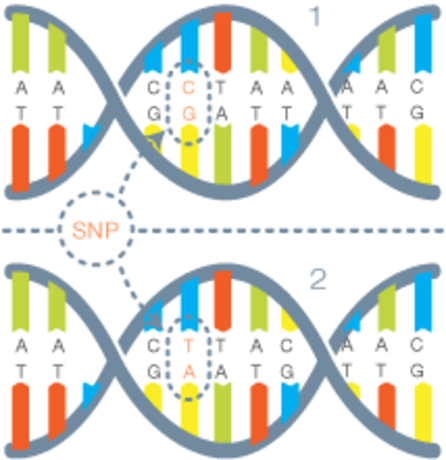
\includegraphics[width=.5\textwidth]{images/snp_diagram} \\
\Tiny \url{http://www.siriusgenomics.com/technology}
\end{center}
\end{frame}

%Slide 5
\begin{frame}{Background Theory}
\framesubtitle{Statistical Models}
  \begin{center}
   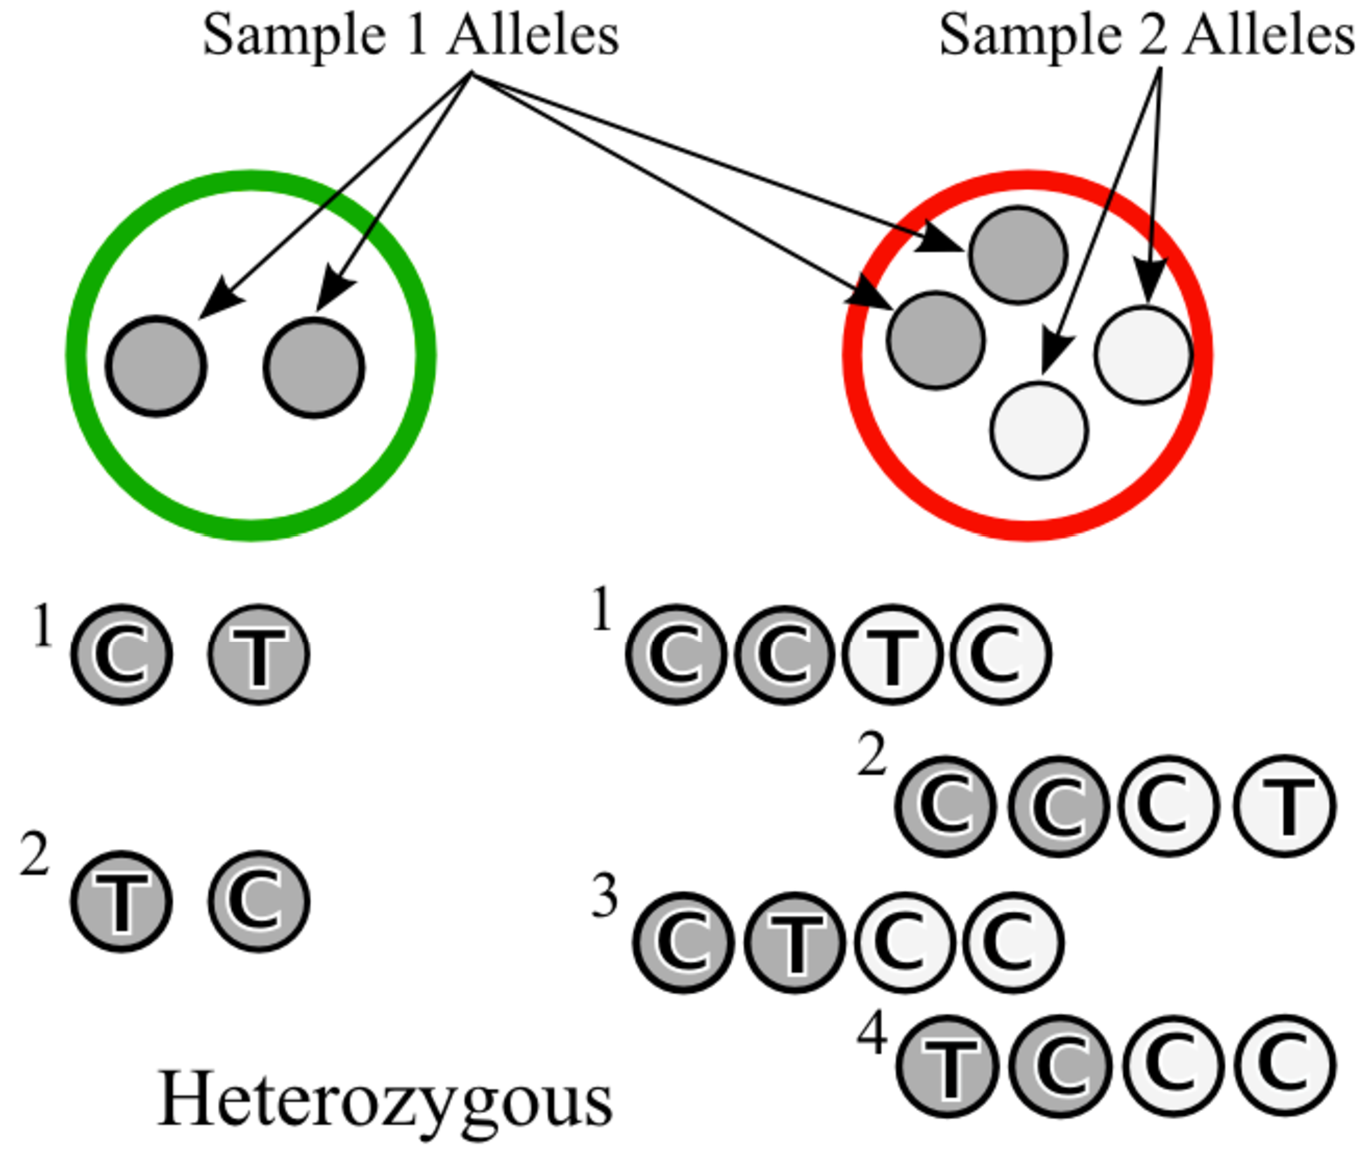
\includegraphics[width=.6\textwidth]{images/hetero_figure2}
  \end{center}
   \begin{itemize}
   	\item contamination identification using the proportion of heterozygous loci
   \end{itemize}
\end{frame}

%Slide 6
\begin{frame}{Background Theory}
\framesubtitle{Bayesian Statistics}
\begin{itemize}
\item Bayesian Inference: Combining new evidence with prior beliefs
	\vspace{1mm}
	\begin{itemize}
	\item $p(H|E) = \frac{p(E|H) \times p(H)}{p(E)}$
	\vspace{2mm}
	\item $posterior \propto likelihood \times prior$
	\vspace{2mm}
	\item $\propto$ means "proportional to"
	\end{itemize}
	\vspace{2mm}
\item Markov chain Monte Carlo (MCMC) methods
	\vspace{1mm}
	\begin{itemize}
	\item algorithms for sampling from probability distributions
	\vspace{2mm}
	\item repeated random sampling to approximate values
	\end{itemize}
\end{itemize}
\end{frame}

%Slide 7
\begin{frame}{Single Population Model}
\begin{columns}[c]

\column{2.25in}
%\begin{itemize}
$\boldsymbol{\rho}$: contamination proportion \\
\vspace{3mm}
$\boldsymbol{z_i}$: contamination indicator \\
\vspace{3mm}
$\boldsymbol{y_{i,\ell}}$: genotype \\
\vspace{3mm}
$\boldsymbol{\theta_{\ell}}$: allele frequency \\
\vspace{3mm}
$\boldsymbol{\alpha}, \pmb{\beta}, \boldsymbol{\lambda}$: Beta distribution parameters \\
\vspace{3mm}
$\boldsymbol{N}$: total \# of individuals \\
\vspace{3mm}
$\boldsymbol{M}$: total \# of loci
%\end{itemize}

\column{2in}
\begin{center}
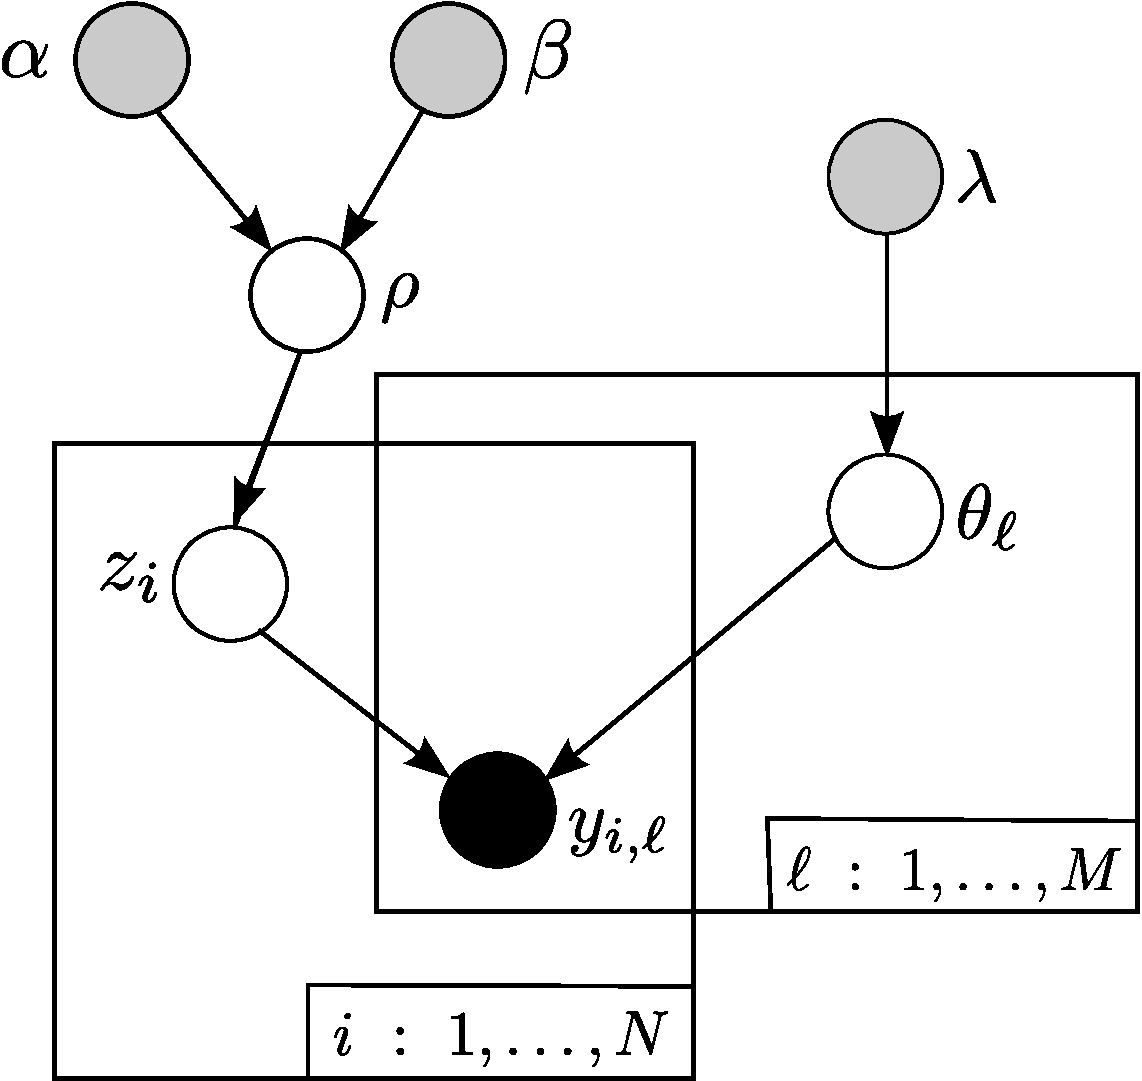
\includegraphics[width=1\textwidth]{images/DAG_1.pdf}
\end{center}
\end{columns}
\end{frame}

%Slide 8
\begin{frame}{Single Population Model}
\framesubtitle{Simulation}
\begin{itemize}
\item Chinook salmon population data from Feather Hatchery Spring-run to used create in silica sample of "fish"
\vspace{3mm}
\item Simulation Parameters
	\begin{itemize}
	\item Number of individuals: $N = 200$
	\vspace{1.5mm}
	\item Number of loci: $L =  (20, 60, 100, 200)$
	\vspace{1.5mm}
	\item Proportion of contaminated samples: $\rho = (0, 0.025, 0.075, 0.2, 0.5)$
	\vspace{1.5mm}
	\item Allele frequencies: $\boldsymbol{\theta} =$ Feather Hatchery frequencies 
	\end{itemize}
	\vspace{3mm}
\item 100 runs of the simulation
\end{itemize}
\end{frame}

%Slide 9
\begin{frame}{Single Population Model}
\framesubtitle{Results}
\begin{columns}[c]

\column{2.75in}
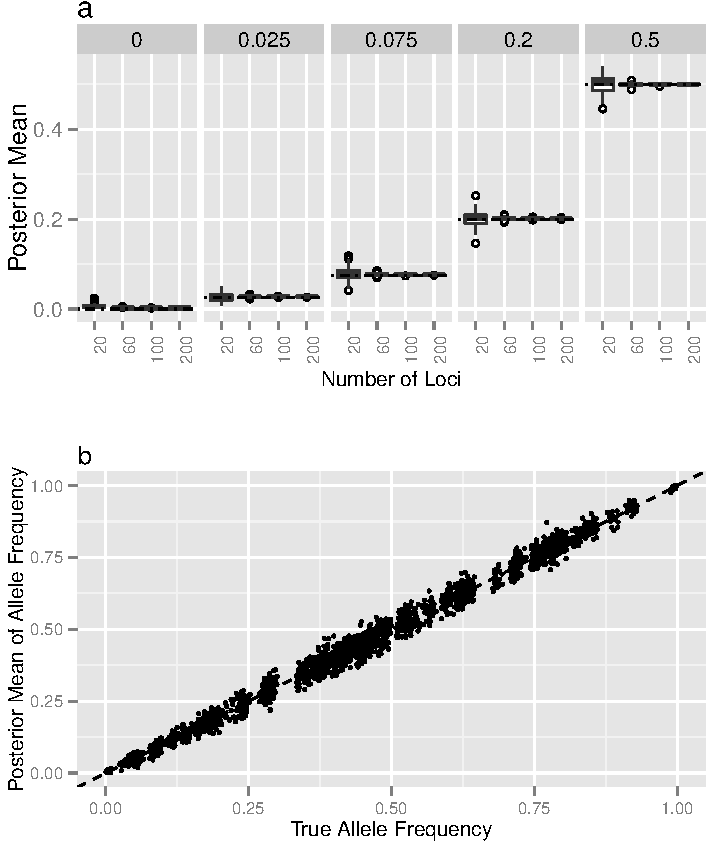
\includegraphics[width=.9\textwidth]{images/rho_and_allele.pdf}

\column{2in}
\begin{itemize}
\item Contamination proportion is estimated well \textbf{(a)}
\vspace{5mm}
\item Good estimation of allele frequencies \textbf{(b)}
\end{itemize}

\end{columns}
\end{frame} 

%Slide 10
\begin{frame}{Single Population Model}
\framesubtitle{Results}
\begin{columns}[c]
\column{2.75in}
\begin{table}
\begin{scriptsize}
\hrule\hrule
\mbox{}\\
{\bf (a)} Contaminated samples 
\begin{center}
\begin{tabular}{lrrrr} 
  &  \multicolumn{4}{c}{\underline{Number of Loci, $L$}} \\
$\rho~~~~~~~$  &  20              &  60              &  100             &  200             \\  
\hline 0.025   &  0.612           &  0.984           &  1.000           &  1.000           \\  
0.075           &  0.765           &  0.990           &  0.999           &  1.000           \\  
0.2             &  0.870           &  0.994           &  1.000           &  1.000           \\  
0.5             &  0.944           &  0.996           &  1.000           &  1.000           \\  
\end{tabular} 
\end{center}
{\bf (b)} Non-contaminated samples 
\begin{center}
\begin{tabular}{lrrrr} 
  &  \multicolumn{4}{c}{\underline{Number of Loci, $L$}} \\
$\rho~~~~~~~$  &  20              &  60              &  100             &  200             \\  
\hline 0       &  0.0010          &  0.0000          &  0.0000          &  0.0000          \\  
0.025           &  0.0030          &  0.0003          &  0.0000          &  0.0000          \\  
0.075           &  0.0124          &  0.0010          &  0.0000          &  0.0000          \\  
0.2             &  0.0239          &  0.0016          &  0.0000          &  0.0000          \\  
0.5             &  0.0618          &  0.0028          &  0.0001          &  0.0000          \\  
\end{tabular} 
\end{center}

\hrule
\end{scriptsize}
\end{table}

\column{2in}
\begin{itemize}
\item true positives \textbf{(a)} and false negatives \textbf{(b)}
\vspace{5mm}
\item almost all contaminated samples identified, with very few false identifications
\end{itemize}
\end{columns}
\end{frame}

%Slide 11
\begin{frame}{Mixture Model}
\begin{columns}[c]

\column{2in}
%\begin{itemize}
$\boldsymbol{\pi}$: mixing proportions \\
\vspace{3mm}
$\boldsymbol{u_i}$: population indicator \\
\vspace{3mm}
$\boldsymbol{B}$: baseline data\\
\vspace{3mm}
$\boldsymbol{\xi}$: Dirichlet distribution parameter
%\end{itemize}

\column{2.25in}
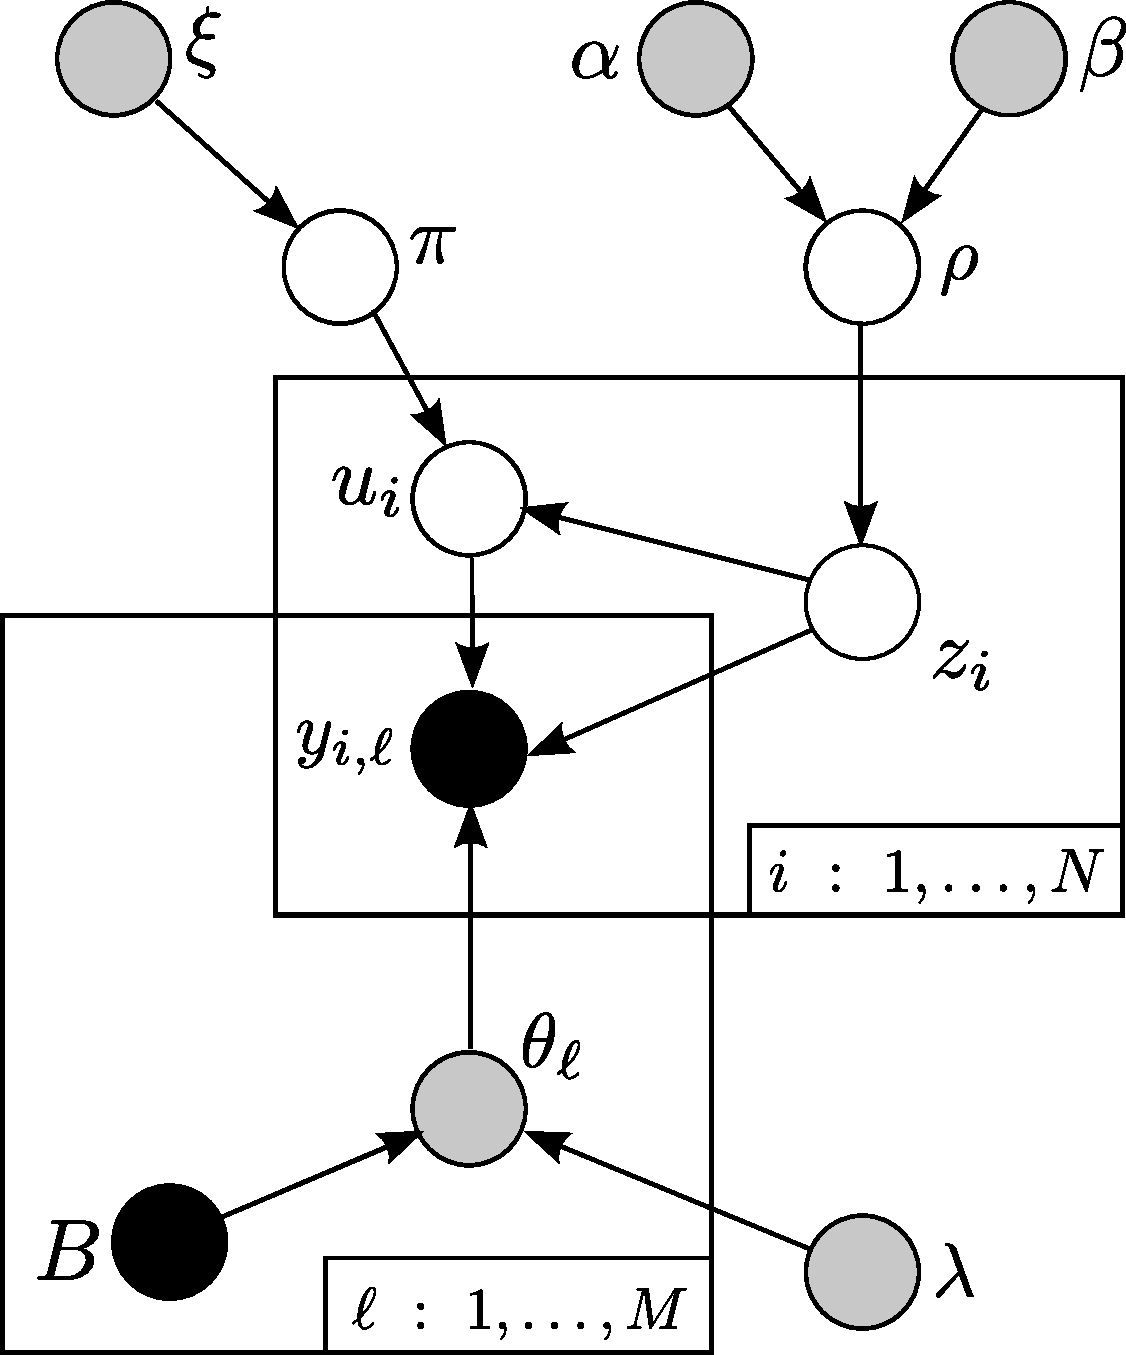
\includegraphics[width=.9\textwidth]{images/DAG_2.pdf}

\end{columns}
\end{frame}

%Slide12
\begin{frame}{Mixture Model}
\framesubtitle{Simulation}
\begin{itemize}
	\item Individuals sampled from existing baseline data
	\vspace{3mm}
	\item Simulation Parameters
	\begin{itemize}
		\item Number of individuals: N = 200
		\vspace{1.5mm}
		\item Proportion of contaminated samples: $\rho = (0, 0.025, 0.075, 0.2, 0.5)$
		\vspace{1.5mm}
		\item Mixing proportions: $\pi = $ 20 sets of observed fishery proportions
	\end{itemize}
	\vspace{3mm}
	\item 20 runs of the simulation
\end{itemize}
\end{frame}

%Slide 13
\begin{frame}{Mixture Model}
\framesubtitle{Results}

\centering
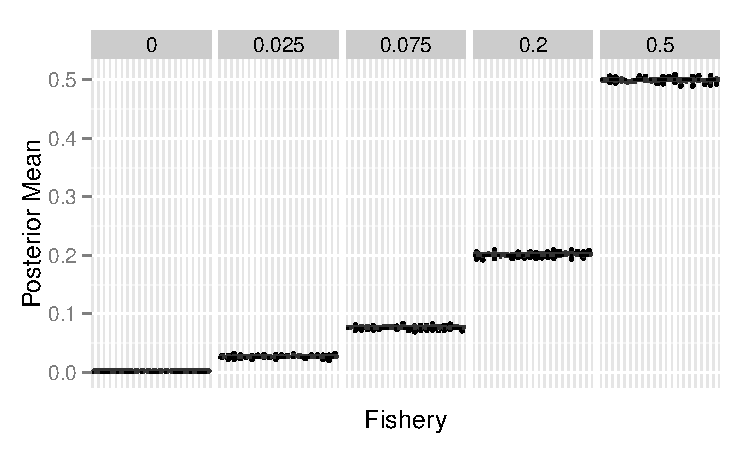
\includegraphics[width=.9\textwidth]{images/mixed_rho.pdf}

\begin{itemize}
	\item Well estimated values for contamination proportion
	\item Nearly all contaminated samples identified
\end{itemize}

\end{frame} 

%Slide 14
\begin{frame}{Conclusion}
\begin{columns}[c]
\column{2.5in}
\centering 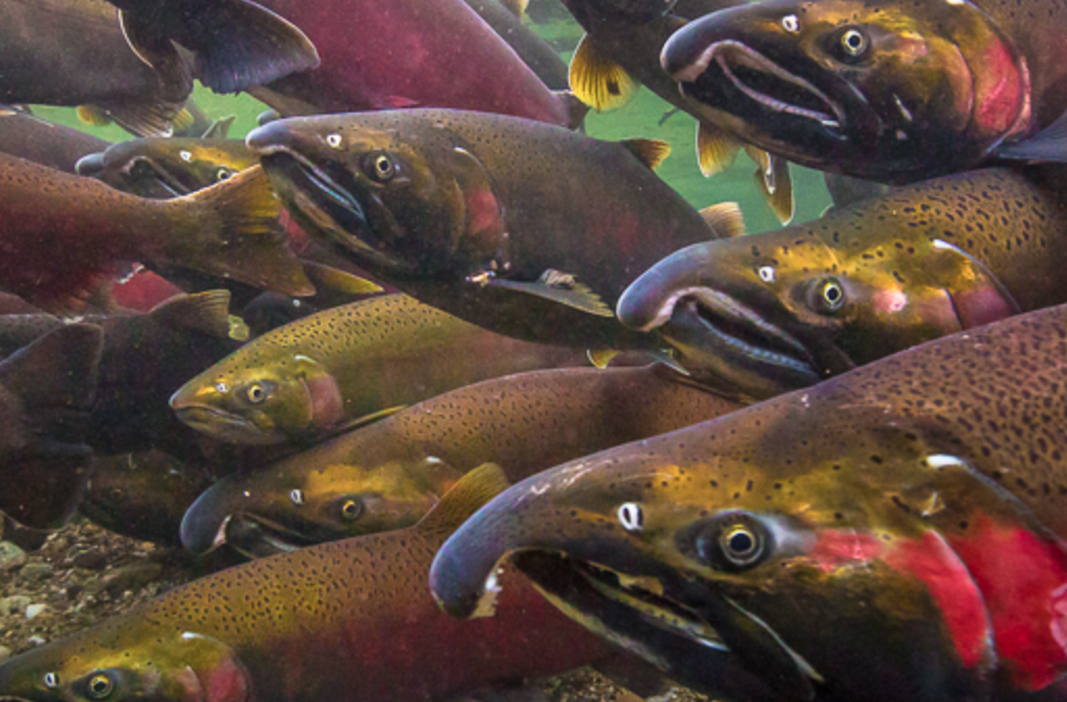
\includegraphics[width=.95\textwidth]{images/conclusion_salmon2.pdf}
\centering \Tiny \url{http://jessicanewley.com/coho-salmon/coho-salmon-2-3/}

\column{2.5in}
\centering 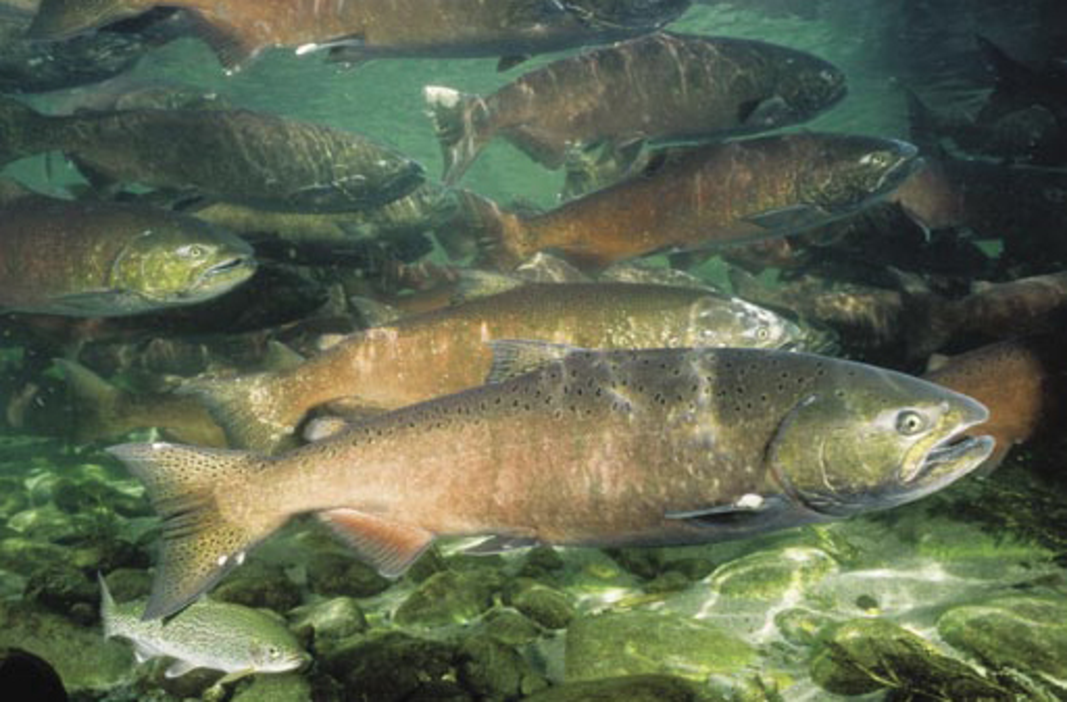
\includegraphics[width=.95\textwidth]{images/conclusion_salmon.pdf} 
\centering \Tiny \url{http://www.wtip.org/drupal/content/friday-fish-report-aug-19}
\end{columns}

\begin{itemize}
   \item Two statistical models and software for inference
   \vspace{3mm}
   \item Contaminated samples identified well using SNPs
\end{itemize}
\end{frame}

%Slide 15
\begin{frame}{Mathematics}
\begin{tiny}
\begin{columns}[T]

\column{2.25in}
\centerline{\textbf{Single Population Model}}
\vspace{2mm}
Prior Distributions \\ \vspace{1mm}
$\bullet \, p(\rho;\alpha,\beta) \propto \rho^{\alpha - 1}(1 - \rho)^{\beta - 1} = Beta(\alpha, \beta)$ \\ \vspace{1mm}
$\bullet \, p(\theta_{\ell};\lambda_{\ell}) \propto \theta_{\ell}^{\lambda_{\ell}-1}(1 - \theta_{\ell})^{\lambda_{\ell}-1} = Beta(\lambda_{\ell},\lambda_{\ell})$ \\ 
\vspace{2mm}

Full Conditional Distributions \\ \vspace{1mm}
$\bullet \, p(z_i=0|\theta_{\ell},y_i,\rho) = \frac{(1-\rho)^{1-z_i}\prod_{\ell=1}^{L} p(y_{\ell}|\theta_{\ell},nocontam)}{R}$ \\ \vspace{1mm}
$\quad p(z_i=1|\theta_{\ell},y_i,\rho) = \frac{\rho^{z_i}\prod_{\ell=1}^{L} p(y_{\ell}|\theta_{\ell},contam)}{R}$ \\ \vspace{1mm}
$\quad R = p(z_i=1|\theta_{\ell},y_i,\rho) + p(z_i = 0|\theta_{\ell},y_i,\rho)$ \\ \vspace{1mm}
$\quad p(y_{\ell}|\theta_{\ell},contam)$ and $p(y_{\ell}|\theta_{\ell},nocontam)$ calculated  \\  \vspace{1mm}
\quad using Hardy Weinberg Equilibrium \\  \vspace{1mm}

$\bullet \, p(\rho|z_i) \propto Beta(\alpha + \sum_{i=1}^{N} z_i, \beta + N - \sum_{i=1}^{N} z_i)$ \\ \vspace{1mm}
$\bullet \,p(\theta_{\ell}|y_{i\ell},z_i) \propto Beta(2x_2 + x_1 + \lambda_{\ell}, 2x_0 + x_1 + \lambda_{\ell})$ \\ \vspace{1mm}
$\quad x_j = \sum_{i:z=0}^{N} \delta(y_{i\ell} = j)$\\

\vspace{3mm}
\centerline{\textbf{Parameters}}
\vspace{2mm}
$\bullet \, \alpha = \beta = \lambda = 0.5$ \\
\vspace{1mm}
$\bullet \, \xi = (\frac{1}{K}, \frac{1}{K}, \ldots, \frac{1}{K})$ where $K = $ number of populations
\vspace{3mm}

\ttiny
GitHub repository \: \url{https://github.com/eriqande/SNPcontam.git} \\
R and Cpp code, manuscript, and presentation \\


\column{2.5in}
\centerline{\textbf{Mixture Model}}
\vspace{2mm}
Prior Distributions \\ \vspace{1mm}
$\bullet \, p(\pi|\xi) \propto \prod_{i = 1}^K \pi_{i}^{\xi_i - 1} = Dirichlet(\xi_1, \ldots, \xi_K)$ \\
\vspace{1mm}
$\bullet \, p(\rho;\alpha,\beta) \propto \rho^{\alpha - 1}(1 - \rho)^{\beta - 1} = Beta(\alpha, \beta)$
$\bullet \, p(\theta_{\ell};\lambda_{\ell}) \propto \theta_{\ell}^{x_i + \lambda_{\ell}-1}(1 - \theta_{\ell})^{x_0 + \lambda_{\ell}-1} = $ \\ 
\vspace{1mm}
$\quad Beta(x_1 + \lambda_{\ell},x_0 + \lambda_{\ell})$ \\ 
\vspace{2mm}

Full Conditional Distributions \\ \vspace{1mm}
$\bullet \, p(z_i=0|\theta,y_i,\rho,B) = \frac{(1-\rho)^{1-z_i}\sum_{k=1}^{K} \prod_{\ell=1}^{L} p(y_{\ell}|\theta_{k,\ell},B,nocontam)}{R}$ \\ 
\vspace{1mm}
$\quad p(z_i=1|\theta,y_i,\rho,B) = \frac{\rho^{z_i}\sum_{k=1}^{K} \prod_{\ell=1}^{L} p(y_{\ell}|\theta_{k,\ell},B,contam)}{R}$ \\
 \vspace{1mm}
$\quad R = p(z_i=1|\theta,y_i,\rho,B) + p(z_i = 0|\theta,y_i,\rho,B)$ \\ 
\vspace{1mm}
$\quad p(y_{\ell} |\theta_{\ell},B,nocontam)$ and $p(y_{\ell} |\theta_{\ell},B,contam)$ calculated \\
\vspace{1mm}
\quad using Polya's Urn model for beta-binomial distribution \\
\vspace{1mm}
$\bullet \, p(u_i = k|\pi,z_i=0,y_i,\theta,B) = \frac{\pi_k \times \prod_{\ell=1}^{L} p(y_{\ell}|\theta_{k,\ell},B,nocontam)}{\sum_{k=1}^{K} \pi_k \times \prod_{\ell=1}^{L} p(y_{\ell}|\theta_{k,\ell},B,nocontam)}$ \\
\vspace{1mm}
$\bullet \, p(\rho|z_i) \propto Beta(\alpha + \sum_{i=1}^{N} z_i, \beta + N - \sum_{i=1}^{N} z_i)$ \\ \vspace{1mm}
$\bullet \, p(\pi|\xi,u_i) \propto Dirichlet(n_1 + \xi_1, \ldots, n_K + \xi_K)$ \\
\vspace{1mm}
$\quad n_k = \sum_{i:z=0}^{N} \delta(u_{i} = k)$
\end{columns}
\end{tiny}
\end{frame} 

\end{document}